\chapter{Stochastic optimal power flow (SOPFLOW)}\label{chap:sopflow}
SOPFLOW solves a stochastic security-constrained multi-period optimal power flow problem. The problem is set up as a two-stage optimization problem where the first-stage (base-case) represents the normal operation of the grid (or the most likely forecast) and the second-stage comprises $N_s$ scenarios of forecast deviation. Each scenario can have multiple contingencies and each contingency can be multi-period.

\section{Formulation}
An illustration of \sopflow is shown in Fig. \ref{fig:sctopflow} for a case with two scenarios $s_0$ and $s_1$ with three contingencies each, and each scenario/contingency with two time-periods. We assume that any contingency is incident at the first time-step, i.e., at $t_0$.


\definecolor{lavander}{cmyk}{0,0.48,0,0}
\definecolor{violet}{cmyk}{0.79,0.88,0,0}
\definecolor{burntorange}{cmyk}{0,0.52,1,0}

\def\lav{lavander!90}
\def\oran{orange!30}

\tikzstyle{contingency}=[draw,circle,violet,bottom color=\lav,
                  top color= white, text=violet,minimum width=50pt]
\tikzstyle{base}=[draw,circle,burntorange, left color=\oran,
                       text=violet,minimum width=50pt]

\tikzstyle{time}=[draw,circle,blue,text=violet,minimum width=2pt]
\tikzstyle{tbase}=[draw,circle,burntorange, left color=\oran,
                            text=violet,minimum width=2pt]
                       
\tikzstyle{cedge}=[color=red]

\begin{figure}[h!]
\centering
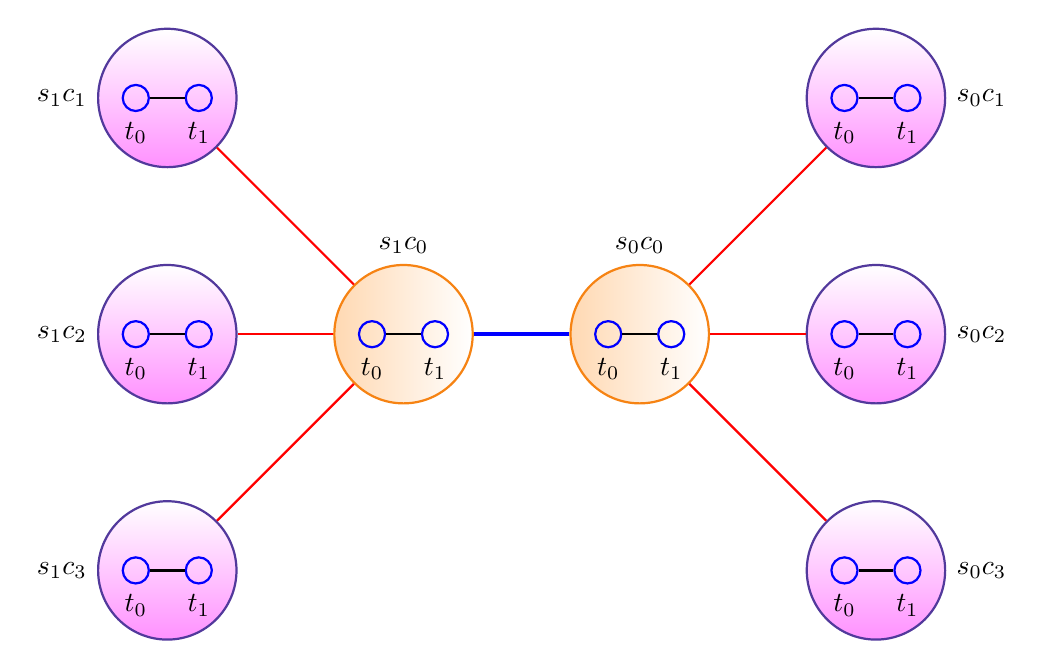
\begin{tikzpicture}[auto, thick]
  % Place base case
  \node[base,label=above:$s_0c_0$] (s0c0) at (1,0) {};
  \node[time,label=below:$t_0$] (s0c0t0) at (0.6,0) {};
  \node[time,label=below:$t_1$] (s0c0t1) at (1.4,0) {};
  
  \node[contingency,label=right:$s_0c_1$] (s0c1) at (4,3) {};
  \node[time,label=below:$t_0$] (s0c1t0) at (3.6,3) {};
  \node[time,label=below:$t_1$] (s0c1t1) at (4.4,3) {};

  \node[contingency,label=right:$s_0c_2$] (s0c2) at (4,0) {};
  \node[time,label=below:$t_0$] (s0c2t0) at (3.6,0) {};
  \node[time,label=below:$t_1$] (s0c2t1) at (4.4,0) {};

  
  \node[contingency,label=right:$s_0c_3$] (s0c3) at (4,-3) {};
  \node[time,label=below:$t_0$] (s0c3t0) at (3.6,-3) {};
  \node[time,label=below:$t_1$] (s0c3t1) at (4.4,-3) {};
  
  \path (s0c0t0) edge (s0c0t1);
  \path (s0c1t0) edge (s0c1t1);
  \path (s0c2t0) edge (s0c2t1);
  \path (s0c3t0) edge (s0c3t1);
  
  \path[cedge] (s0c0) edge (s0c1);
  \path[cedge] (s0c0) edge (s0c2);
  \path[cedge] (s0c0) edge (s0c3);

  % Second scenario
  \node[base,label=above:$s_1c_0$] (s1c0) at (-2,0) {};
  \node[time,label=below:$t_0$] (s1c0t0) at (-2.4,0) {};
  \node[time,label=below:$t_1$] (s1c0t1) at (-1.6,0) {};
  
  \node[contingency,label=left:$s_1c_1$] (s1c1) at (-5,3) {};
  \node[time,label=below:$t_0$] (s1c1t0) at (-5.4,3) {};
  \node[time,label=below:$t_1$] (s1c1t1) at (-4.6,3) {};

  \node[contingency,label=left:$s_1c_2$] (s1c2) at (-5,0) {};
  \node[time,label=below:$t_0$] (s1c2t0) at (-5.4,0) {};
  \node[time,label=below:$t_1$] (s1c2t1) at (-4.6,0) {};

  
  \node[contingency,label=left:$s_1c_3$] (s1c3) at (-5,-3) {};
  \node[time,label=below:$t_0$] (s1c3t0) at (-5.4,-3) {};
  \node[time,label=below:$t_1$] (s1c3t1) at (-4.6,-3) {};
  
  \path (s1c0t0) edge (s1c0t1);
  \path (s1c1t0) edge (s1c1t1);
  \path (s1c2t0) edge (s1c2t1);
  \path (s1c3t0) edge (s1c3t1);
  
  \path[cedge] (s1c0) edge (s1c1);
  \path[cedge] (s1c0) edge (s1c2);
  \path[cedge] (s1c0) edge (s1c3);

  \path (s0c0) edge [ultra thick,color=blue] (s1c0);

\end{tikzpicture}

\caption{Stochastic multi-period contingency constrained structure with two scenarios $s_0$ and $s_1$. Each scenario has three contingencies $c_1$,$c_2$,and $c_3$. $s_0c_0$ and $s_1c_0$ denote the base-cases for the two scenarios. Each scenario and contingency has two time-periods $t_0$, and $t_2$, $t_2$. The {\textcolor{red}{red}} line denotes the coupling between the contingencies and their respective base-case scenarios.The {\textcolor{blue}{blue}} line denotes the coupling between the scenarios}
\label{fig:sctopflow}
\end{figure}


The full formulation for the stochastic security-constrained multi-period optimal power flow is given in (\ref{eq:sctopflow_start}) -- (\ref{eq:sctopflow_end}). In this formulation, the objective is to reduce the expected cost, where $f(x_{s,c,t})$ is the cost for scenario $s$ with contingency $c$ at time $t$. $\pi_s$ is the probability of scenario $s$.

\begin{align}
\centering
\text{min}&~\sum_{s=0}^{N_s-1}\pi_s\sum_{c=0}^{N_c-1}\sum_{t=0}^{N_t-1}f(x_{s,c,t})&  \label{eq:sctopflow_start}\\
&\text{s.t.}& \nonumber \\
&~g(x_{s,c,t}) = 0,                                        &s \in \left[1,N_s-1\right],c \in \left[0,N_c-1\right], t \in \left[0,N_t-1\right]& \\
&~h(x_{s,c,t}) \le 0,                                      &s \in \left[1,N_s-1\right],c \in \left[0,N_c-1\right], t \in \left[0,N_t-1\right]& \\
x^- & \le x_{s,c,t} \le x^+,                               &s \in \left[1,N_s-1\right],c \in \left[0,N_c-1\right], t\in \left[0,N_t-1\right]& \\
-\Delta x_t & \le x_{s,c,t} - x_{s,c,t-\Delta{t}} \le \Delta x_t,&s \in \left[1,N_s-1\right],c \in \left[0,N_c-1\right], t \in \left[1,N_t-1\right]& \label{eq:sctopflow_time_coupling}\\
-\Delta x_c & \le x_{s,c,0} - x_{s,0,0} \le \Delta x_c,&s \in \left[1,N_s-1\right],c \in \left[1,N_c-1\right]&
\label{eq:sctopflow_contingency_coupling} \\
-\Delta x_s & \le x_{s,0,0} - x_{0,0,0} \le \Delta x_s,&s \in \left[1,N_s-1\right]&
\label{eq:sctopflow_end}
\end{align}

The modeling details used for an optimial power flow problem are also used for a {\sopflow} problem, i.e., each of the circles shown in Fig. \ref{fig:sctopflow} has the modeling details of an optimal power flow problem (\opflow). Incorporating the probabilities $\pi_s$ for each scenario is not implemented yet which leads to each scenario having an equal probability. 

Depending on the options selected, SOPFLOW can be used to solve 
\begin{itemize}
    \item Single-period stochastic optimal power flow : No contingencies or time-periods
    \item Single-period contingency-constrained stochastic optimal power flow : No time-periods
    \item Multi-period security-constrained stochastic optimal power flow : Full formulation
\end{itemize}

Currently, \sopflow uses wind power generation as the stochastic variables and each scenario is a realization of the power output from wind generators. A zero fuel cost is used for wind power generation to ensure wind generation would be the dispatched to the given target level (upper limit). 

For the contingecy-constrained stochastic optimal power flow, \sopflow flattens out the contingencies and scenarios to a two-level formulation. In this formulation, all the scenarios (and their contingencies) are coupled to a base scenario problem.

For contingencies, \sopflow supports generation and/or transmission outages. A contingency can have multiple outages, but, it should not cause any islanding. The coupling between the no-contingency and the contingency case for each scenario is also the difference in real power output ($p_{jsct}^{\text{g}} - p_{js0t}^{\text{g}},~ \jinJgen$) that must be within the 30 minute generator ramp rate. Refer to \ref{chap:scopflow} for details on the contingency modeling.

For multi time-period, we use ramping constraints on the generator real power output between successive time steps.

\sopflow can be run in two modes: preventive and corrective. In the preventive mode, generator real power output is fixed to the base-case values for generators at PV bus(es). In this mode, the generators at the reference bus provide/absorb any deficit/surplus power. The corrective mode allows deviation of the PV and PQ generator real power from the base-case dispatch constrained by its 30-min. ramp rate capability. Note that the preventive/corrective mode is only applied at the first step $t_0$. In the successive time-steps, the generator dispatch is dictated by the previous step dispatch and the ramp limits.

\section{Solvers}
\sopflow supports solving the optimization problem via \ipopt, \hiop, or \emph{EMPAR}. \ipopt can solve \sopflow on single rank only. \hiop supports solving the problem in parallel using a primal-decomposition algorithm. With HiOp, one can solve the subproblem either on the CPU or GPU by selecting the appropriate subproblem model and solver (see options table below). However, note that \emph{ExaGO needs to be built with \ipopt even when using \hiop solver.} The \emph{EMPAR} solver does not solve the stochastic ACOPF problem, but it only solves the base-case and the stochastic scenarios independently with \opflow. It distributes the scenarios and contingencies to different processes when executed in parallel. Table \ref{tab:sopflow_solvers} lists the compatibility of the different solvers for different variations of \sopflow.

\begin{center}
\begin{table}[!htbp]
    \centering
    \caption{\sopflow solver compatibility}
    \begin{tabular}{|c|c|c|c|}
      \hline
      \textbf{Solver} & \textbf{Stochastic scenarios} & \textbf{Include contingencies} & \textbf{Include multi-period} \\
      \hline
      IPOPT   & Y & Y & Y \\ \hline
      HIOP & Y & Y  & N \\ \hline
      EMPAR  & Y & Y  & Y \\ \hline
    \end{tabular}
    \label{tab:sopflow_solvers}
\end{table}
\end{center}


\section{Input and Output}
The following files are needed for executing SOPFLOW.
\begin{itemize}
    \item \textbf{Network file:} The network file describing the network details. Only \matpower format files are currently supported.
    \item \textbf{Scenario file:} \sopflow only supports reading wind generation scenarios in a CSV format. An example of this format for the 9-bus case is \href{https://gitlab.pnnl.gov/exasgd/frameworks/exago/-/tree/master/datafiles/case9/scenarios_9bus.csv}{here}.
    \item \textbf{Contingency file:} Contingencies can be specified via PTI format file as described in chapter \ref{chap:scopflow}. The option \lstinline{-sopflow_enable_multicontingency} should be set for multi-contingency problems.
    \item \textbf{Load data:} One file for load real power and one for reactive power. The files need to be in CSV format. An example of the format for the 9-bus case is \href{https://gitlab.pnnl.gov/exasgd/frameworks/exago/-/tree/master/datafiles/case9}{here}.
\end{itemize}

The \sopflow output is saved to a directory named \texttt{sopflowout}. This
directory contains $N_s$ subdirectories to save the solution for each scenario.
Each of these subdirectories contain $N_c$ subdirectories, one for each
contingency. Each contingency subdirectory has $N_t$ MATPOWER format files to
store the output for each time-period for the given contingency and scenario.
The subdirectories have the directory name format \texttt{scen_x} where x is
the scenario number,  \texttt{cont_y} where y is the contingency number, and
the output files have the file name format \texttt{t_z} where z is the time-step number.

\section{Usage}
\begin{lstlisting}
    ./sopflow -netfile <netfilename>  -windgen <wind_scenario_filename> \
    [-sopflow_enable_multicontingency 1] <sopflowoptions>
\end{lstlisting}

\section{Options}

\begin{table}[H]
  \caption{SOPFLOW options}
  \small
  \begin{tabular}{|p{0.3\textwidth}|p{0.2\textwidth}|p{0.3\textwidth}|p{0.2\textwidth}|}
    \hline
    \textbf{Option} & \textbf{Meaning} & \textbf{Values (Default value)} & \textbf{Compatibility} \\ \hline
    -netfile & Network file name & string 4096 characters (\href{https://gitlab.pnnl.gov/exasgd/frameworks/exago/-/blob/master/datafiles/case9/case9mod_gen3_wind.m}{case9mod\_gen3\_wind.m}) &\\ \hline
    -windgen & Scenario file name & string 4096 characters (\href{https://gitlab.pnnl.gov/exasgd/frameworks/exago/-/blob/master/datafiles/case9/10scenarios_9bus.csv}{case9/10scenarios\_9bus.csv}) &\\ \hline
    -ctgcfile & Contingency file name & string (\href{https://gitlab.pnnl.gov/exasgd/frameworks/exago/-/blob/master/datafiles/case9/case9.cont}{case9.cont}) &\\ \hline
    -save\_output & Save output to directory & 0 or 1 (0) & Format determined by OPFLOW option. \\ \hline
    -sopflow\_output\_directory & Output directory path & ``sopflowout'' & \\ \hline
    -sopflow\_mode & Operation mode: Preventive or corrective & 0 or 1 (0) &\\ \hline
    -sopflow\_model & Set model for SOPFLOW & GENRAMP, GENRAMPC (GENRAMP) &\\ \hline
    -sopflow\_solver & Set solver for SOPFLOW & IPOPT, HIOP, or  EMPAR &\\ \hline
    -sopflow\_subproblem\_solver & Set solver for subproblem & IPOPT or HIOP (IPOPT) &Only when using HiOp solver for SOPFLOW \\ \hline
    -sopflow\_subproblem\_model & Set model for subproblem & See OPFLOW chapter &Only when using HiOp solver for SOPFLOW \\ \hline
    -sopflow\_enable\_multicontingency & Multi-contingency SOPFLOW & 0 or 1 (0) &\\ \hline
    -sopflow\_flatten\_contingencies & Flatten contingencies for SOPFLOW & 0 or 1 (1) &\\ \hline
    -sopflow\_Ns & Number of scenarios & int (Default 0. Use -1 to select all scenarios from the scenario file) &\\ \hline
    -sopflow\_Nc & Number of contingencies & int (0. Passing -1 results in all contingencies in the file used) &\\ \hline
  \end{tabular}
  \label{tab:sopflow_options}
\end{table}

%See table \ref{tab:sopflow_options}. With multi-contingency SOPFLOW, all \scopflow options given in Table \ref{tab:scopflow_options} can be used to tune the contingencies. All \opflow options in Table \ref{tab:opflow_options}, along with \tcopflow options in Table \ref{tab:tcopflow_options} can also be used. Multi-contingency SOPFLOW also allows the options listed after -sopflow\_enable\_multicontingency in Table \ref{tab:sopflow_options} to be used.

\section{Examples}
Some \sopflow example runs are provided with some sample output. Options are the default options given in Tables \ref{tab:opflow_options}, \ref{tab:tcopflow_options}, \ref{tab:scopflow_options} and \ref{tab:sopflow_options} unless otherwise specified. Sample output is generated by running examples in the installation directory.

Example using the \ipopt solver:

\begin{lstlisting}
bin/sopflow -netfile $EXAGO_DIR/datafiles/case9/case9mod.m -windgen $EXAGO_DIR/datafiles/case9/10_scenarios_9bus.csv -sopflow_Ns 4 -sopflow_enable_multicontingency 0 -sopflow_solver IPOPT -print_output
[ExaGO] SOPFLOW: Application created
Rank[0],s = 0, scen_num = 0
Rank[0],s = 1, scen_num = 1
Rank[0],s = 2, scen_num = 2
Rank[0],s = 3, scen_num = 3
[ExaGO] SOPFLOW: Using IPOPT solver
[ExaGO] SOPFLOW: Setup completed

******************************************************************************
This program contains Ipopt, a library for large-scale nonlinear optimization.
 Ipopt is released as open source code under the Eclipse Public License (EPL).
         For more information visit http://projects.coin-or.org/Ipopt
******************************************************************************

This is Ipopt version 3.12.10, running with linear solver ma27.

Number of nonzeros in equality constraint Jacobian...:      513
Number of nonzeros in inequality constraint Jacobian.:      288
Number of nonzeros in Lagrangian Hessian.............:      564

Total number of variables............................:      120
                     variables with only lower bounds:        0
                variables with lower and upper bounds:       88
                     variables with only upper bounds:        0
Total number of equality constraints.................:       96
Total number of inequality constraints...............:       72
        inequality constraints with only lower bounds:        0
   inequality constraints with lower and upper bounds:       72
        inequality constraints with only upper bounds:        0

iter    objective    inf_pr   inf_du lg(mu)  ||d||  lg(rg) alpha_du alpha_pr  ls
   0  3.2548812e+04 1.80e+00 1.00e+02  -1.0 0.00e+00    -  0.00e+00 0.00e+00   0
   1  2.6023632e+04 1.18e+00 1.21e+02  -1.0 1.07e+00    -  5.64e-02 3.40e-01f  1
   2  2.0106844e+04 4.83e-01 2.57e+03  -1.0 6.99e-01   2.0 1.02e-02 6.07e-01f  1
   3  2.0011119e+04 4.70e-01 2.50e+03  -1.0 5.84e-01   2.4 1.32e-01 2.67e-02f  1
   4  1.9372689e+04 3.88e-01 1.99e+03  -1.0 7.94e-01   1.9 2.37e-01 1.97e-01f  1
   ...
  18  1.6587232e+04 4.15e-05 1.21e+03  -5.7 5.76e-03    -  1.00e+00 9.18e-01h  1
  19  1.6587229e+04 8.62e-06 1.55e-05  -5.7 3.00e-03    -  1.00e+00 1.00e+00h  1
iter    objective    inf_pr   inf_du lg(mu)  ||d||  lg(rg) alpha_du alpha_pr  ls
  20  1.6587228e+04 1.50e-06 2.56e-06  -7.0 1.25e-03    -  1.00e+00 1.00e+00h  1
  21  1.6587228e+04 2.18e-07 4.53e-07  -7.0 4.77e-04    -  1.00e+00 1.00e+00h  1

Number of Iterations....: 21

                                   (scaled)                 (unscaled)
Objective...............:   3.7191094895317639e+02    1.6587228323311669e+04
Dual infeasibility......:   4.5286779256921672e-07    2.0197903548587065e-05
Constraint violation....:   3.6703967934426096e-08    3.6703967934426096e-08
Complementarity.........:   6.2406713469536533e-07    2.7833394207413294e-05
Overall NLP error.......:   6.2406713469536533e-07    2.7833394207413294e-05


Number of objective function evaluations             = 22
Number of objective gradient evaluations             = 22
Number of equality constraint evaluations            = 22
Number of inequality constraint evaluations          = 22
Number of equality constraint Jacobian evaluations   = 22
Number of inequality constraint Jacobian evaluations = 22
Number of Lagrangian Hessian evaluations             = 21
Total CPU secs in IPOPT (w/o function evaluations)   =      0.043
Total CPU secs in NLP function evaluations           =      0.013

EXIT: Optimal Solution Found.
=============================================================
Stochastic Optimal Power Flow
=============================================================
Number of scenarios                 4
Multi-contingency scenarios?        NO
Solver                              IPOPT
Initialization                      MIDPOINT
Load loss allowed                   NO
Power imbalance allowed             NO
Ignore line flow constraints        NO

Convergence status                  CONVERGED
Objective value (base)              4149.15

----------------------------------------------------------------------
Bus        Pd      Qd      Vm      Va      mult_Pmis      mult_Qmis      Pslack         Qslack        
----------------------------------------------------------------------
1         0.00    0.00   1.100   0.000      2152.67         0.00         0.00         0.00
2         0.00    0.00   1.095   3.935      2108.81        -0.00         0.00         0.00
3         0.00    0.00   1.087   1.637      2117.68        -0.00         0.00         0.00
4         0.00    0.00   1.097  -2.054      2152.95         0.18         0.00         0.00
5        75.00   50.00   1.079  -3.127      2163.77         7.53         0.00         0.00
6        90.00   30.00   1.087  -4.084      2181.34         1.69         0.00         0.00
7         0.00    0.00   1.100   0.455      2109.21        -0.04         0.00         0.00
8       100.00   35.00   1.089  -1.907      2130.61         3.09         0.00         0.00
9         0.00    0.00   1.100  -0.471      2117.94        -0.09         0.00         0.00

----------------------------------------------------------------------------------------
From       To       Status     Sft      Stf     Slim     mult_Sf  mult_St 
----------------------------------------------------------------------------------------
1          4          1       75.41    75.22   380.00    -0.00    -0.00
2          7          1      117.10   117.61   250.00    -0.00    -0.00
3          9          1       78.55    79.51   300.00    -0.00    -0.00
4          5          1       29.85    40.63   250.00    -0.00    -0.00
4          6          1       46.99    47.91   250.00    -0.00    -0.00
5          7          1       51.14    48.90   250.00    -0.00    -0.00
6          9          1       47.20    49.41   150.00    -0.00    -0.00
7          8          1       69.69    70.99   250.00    -0.00    -0.00
8          9          1       36.50    31.07   150.00    -0.00    -0.00

----------------------------------------------------------------------------------------
Gen      Status     Fuel     Pg       Qg       Pmin     Pmax     Qmin     Qmax  
----------------------------------------------------------------------------------------
1          1    UNDEFINED    75.12     6.61    10.00   350.00  -300.00   300.00
2          1    UNDEFINED   116.99    -5.04    10.00   300.00  -300.00   300.00
3          1    UNDEFINED    75.00   -23.36    10.00    85.00  -300.00   300.00
[ExaGO] Finalizing sopflow application.
\end{lstlisting}

Example using the \emph{IPOPT} solver with multicontingency enabled:

\begin{lstlisting}
bin/sopflow -netfile $EXAGO_DIR/datafiles/case9/case9mod.m -windgen $EXAGO_DIR/datafiles/case9/10_scenarios_9bus.csv -sopflow_Ns 4 -sopflow_enable_multicontingency 1 -sopflow_solver IPOPT -print_output -sopflow_Nc 4 -ctgcfile $EXAGO_DIR/datafiles/case9/case9.cont -sopflow_Nc 4
[ExaGO] SOPFLOW: Application created
Rank[0],s = 0, scen_num = 0, cont_num = 0
Rank[0],s = 1, scen_num = 0, cont_num = 1
Rank[0],s = 2, scen_num = 0, cont_num = 2
Rank[0],s = 3, scen_num = 0, cont_num = 3
Rank[0],s = 4, scen_num = 0, cont_num = 4
Rank[0],s = 5, scen_num = 1, cont_num = 0
Rank[0],s = 6, scen_num = 1, cont_num = 1
Rank[0],s = 7, scen_num = 1, cont_num = 2
Rank[0],s = 8, scen_num = 1, cont_num = 3
Rank[0],s = 9, scen_num = 1, cont_num = 4
Rank[0],s = 10, scen_num = 2, cont_num = 0
Rank[0],s = 11, scen_num = 2, cont_num = 1
Rank[0],s = 12, scen_num = 2, cont_num = 2
Rank[0],s = 13, scen_num = 2, cont_num = 3
Rank[0],s = 14, scen_num = 2, cont_num = 4
Rank[0],s = 15, scen_num = 3, cont_num = 0
Rank[0],s = 16, scen_num = 3, cont_num = 1
Rank[0],s = 17, scen_num = 3, cont_num = 2
Rank[0],s = 18, scen_num = 3, cont_num = 3
Rank[0],s = 19, scen_num = 3, cont_num = 4
[ExaGO] SOPFLOW: Using IPOPT solver
[ExaGO] SOPFLOW: Setup completed

******************************************************************************
This program contains Ipopt, a library for large-scale nonlinear optimization.
 Ipopt is released as open source code under the Eclipse Public License (EPL).
         For more information visit http://projects.coin-or.org/Ipopt
******************************************************************************

This is Ipopt version 3.12.10, running with linear solver ma27.

Number of nonzeros in equality constraint Jacobian...:     2449
Number of nonzeros in inequality constraint Jacobian.:     1312
Number of nonzeros in Lagrangian Hessian.............:     2820

Total number of variables............................:      600
                     variables with only lower bounds:        0
                variables with lower and upper bounds:      440
                     variables with only upper bounds:        0
Total number of equality constraints.................:      480
Total number of inequality constraints...............:      328
        inequality constraints with only lower bounds:        0
   inequality constraints with lower and upper bounds:      328
        inequality constraints with only upper bounds:        0

iter    objective    inf_pr   inf_du lg(mu)  ||d||  lg(rg) alpha_du alpha_pr  ls
   0  1.6274406e+05 1.80e+00 1.00e+02  -1.0 0.00e+00    -  0.00e+00 0.00e+00   0
   1  1.4901965e+05 1.56e+00 8.69e+01  -1.0 1.07e+00    -  1.73e-01 1.31e-01f  1
   2  1.4480394e+05 1.49e+00 1.32e+02  -1.0 1.80e+00    -  1.34e-03 4.72e-02f  1
   3  1.3529809e+05 1.31e+00 1.15e+02  -1.0 1.22e+00    -  4.90e-02 1.18e-01f  1
   4  1.1656024e+05 9.25e-01 9.13e+01  -1.0 8.50e-01    -  9.55e-02 2.99e-01f  1
   5  1.0783333e+05 7.18e-01 9.48e+01  -1.7 7.97e-01    -  2.05e-01 2.24e-01f  1
   6  9.9954510e+04 5.10e-01 9.64e+01  -1.7 7.94e-01    -  3.55e-01 2.89e-01f  1
   7  9.3292251e+04 3.16e-01 9.31e+01  -1.7 7.35e-01    -  3.05e-01 3.78e-01f  1
   8  9.2973069e+04 3.05e-01 9.00e+01  -1.7 4.70e-01   2.0 3.84e-02 3.33e-02f  1
   ...
  30  8.3618318e+04 1.07e-05 1.74e+03  -5.7 3.88e-03    -  1.00e+00 8.83e-01f  1
  31  8.3618280e+04 5.27e-06 2.36e-04  -5.7 2.35e-03    -  1.00e+00 1.00e+00h  1
  32  8.3618280e+04 6.40e-07 1.28e-06  -5.7 8.17e-04    -  1.00e+00 1.00e+00h  1
  33  8.3618274e+04 1.95e-07 1.70e-06  -7.0 4.52e-04    -  1.00e+00 1.00e+00h  1
  34  8.3618274e+04 8.21e-09 1.71e-08  -7.0 9.25e-05    -  1.00e+00 1.00e+00h  1

Number of Iterations....: 34

                                   (scaled)                 (unscaled)
Objective...............:   1.8748492036555979e+03    8.3618274483039670e+04
Dual infeasibility......:   1.7101740512915904e-08    7.6273762687604936e-07
Constraint violation....:   1.3811524007811826e-09    1.3811524007811826e-09
Complementarity.........:   1.1101524615042143e-07    4.9512799783087964e-06
Overall NLP error.......:   1.1101524615042143e-07    4.9512799783087964e-06


Number of objective function evaluations             = 35
Number of objective gradient evaluations             = 35
Number of equality constraint evaluations            = 35
Number of inequality constraint evaluations          = 35
Number of equality constraint Jacobian evaluations   = 35
Number of inequality constraint Jacobian evaluations = 35
Number of Lagrangian Hessian evaluations             = 34
Total CPU secs in IPOPT (w/o function evaluations)   =      0.135
Total CPU secs in NLP function evaluations           =      0.094

EXIT: Optimal Solution Found.
=============================================================
Stochastic Optimal Power Flow
=============================================================
Number of scenarios                 4
Multi-contingency scenarios?        YES
Contingencies per scenario          4
Solver                              IPOPT
Initialization                      MIDPOINT
Load loss allowed                   NO
Power imbalance allowed             NO
Ignore line flow constraints        NO

Convergence status                  CONVERGED
Objective value (base)              4149.15

----------------------------------------------------------------------
Bus        Pd      Qd      Vm      Va      mult_Pmis      mult_Qmis      Pslack         Qslack        
----------------------------------------------------------------------
1         0.00    0.00   1.100   0.000      2152.67         0.00         0.00         0.00
2         0.00    0.00   1.095   3.935      2108.81        -0.00         0.00         0.00
3         0.00    0.00   1.087   1.637      2117.68        -0.00         0.00         0.00
4         0.00    0.00   1.097  -2.054      2152.95         0.18         0.00         0.00
5        75.00   50.00   1.079  -3.127      2163.77         7.53         0.00         0.00
6        90.00   30.00   1.087  -4.084      2181.34         1.69         0.00         0.00
7         0.00    0.00   1.100   0.455      2109.22        -0.04         0.00         0.00
8       100.00   35.00   1.089  -1.907      2130.61         3.09         0.00         0.00
9         0.00    0.00   1.100  -0.471      2117.94        -0.09         0.00         0.00

----------------------------------------------------------------------------------------
From       To       Status     Sft      Stf     Slim     mult_Sf  mult_St 
----------------------------------------------------------------------------------------
1          4          1       75.41    75.22   380.00    -0.00    -0.00
2          7          1      117.10   117.61   250.00    -0.00    -0.00
3          9          1       78.55    79.51   300.00    -0.00    -0.00
4          5          1       29.85    40.63   250.00    -0.00    -0.00
4          6          1       46.99    47.91   250.00    -0.00    -0.00
5          7          1       51.14    48.90   250.00    -0.00    -0.00
6          9          1       47.20    49.41   150.00    -0.00    -0.00
7          8          1       69.69    70.99   250.00    -0.00    -0.00
8          9          1       36.50    31.07   150.00    -0.00    -0.00

----------------------------------------------------------------------------------------
Gen      Status     Fuel     Pg       Qg       Pmin     Pmax     Qmin     Qmax  
----------------------------------------------------------------------------------------
1          1    UNDEFINED    75.12     6.61    10.00   350.00  -300.00   300.00
2          1    UNDEFINED   116.99    -5.04    10.00   300.00  -300.00   300.00
3          1    UNDEFINED    75.00   -23.36    10.00    85.00  -300.00   300.00
[ExaGO] Finalizing sopflow application.
\end{lstlisting}
